\begin{frame}[fragile]{Problem 1: Two-Pointer Approach}
    \textbf{Problem:} Find indices of two numbers in a \textbf{sorted} array that sum to a target.

    \begin{columns}[T]
        \begin{column}{0.45\textwidth}
            \begin{block}{The Algorithm}
            \small
            \begin{enumerate}
                \item Initialize $i = 0, j = n-1$
                \item Calculate $sum = nums[i] + nums[j]$
                \item If $sum == target$, return indices.
                \item If $sum < target$, move $i \rightarrow$
                \item If $sum > target$, move $j \leftarrow$
            \end{enumerate}
            \end{block}
            
            \begin{block}{Complexity}
            \small
            \begin{itemize}
                \item \textbf{Time:} $O(N)$
                \item \textbf{Space:} $O(1)$
            \end{itemize}
            \end{block}
        \end{column}

        \begin{column}{0.52\textwidth}
            \begin{exampleblock}{Kotlin Implementation}
\begin{lstlisting}[language=Kotlin, basicstyle=\tiny\ttfamily, keywordstyle=\color{blue}]
fun twoSum(nums: IntArray, target: Int): IntArray {
    var i = 0
    var j = nums.size - 1
    
    while (i < j) {
        val sum = nums[i] + nums[j]
        when {
            sum == target -> return intArrayOf(i, j)
            sum < target -> i++
            else -> j--
        }
    }
    return intArrayOf()
}
\end{lstlisting}
            \end{exampleblock}
        \end{column}
    \end{columns}
\end{frame}
\begin{frame}{Two Sum: Visual Trace}
    \centering
    \textbf{Target = 35}

    % Iteration 1
    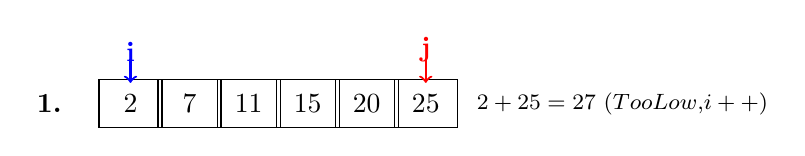
\begin{tikzpicture}[scale=0.75]
        \node[left] at (-0.5,0.35) {\textbf{1.}};
        \foreach \x/\val in {0/2,1/7,2/11,3/15,4/20,5/25}
            \node[draw, minimum width=0.8cm, minimum height=0.6cm] at (\x+0.5,0.35) {\val};
        \draw[->, blue, thick] (0.5,1.1) -- (0.5,0.7) node[above=4pt] {\bf i};
        \draw[->, red, thick] (5.5,1.1) -- (5.5,0.7) node[above=4pt] {\bf j};
        \node[right] at (6.2, 0.35) {\footnotesize $2+25=27 \ (\text{Too Low, } i++)$};
    \end{tikzpicture}

    \pause
    \vspace{0.2cm}
    % Iteration 2
    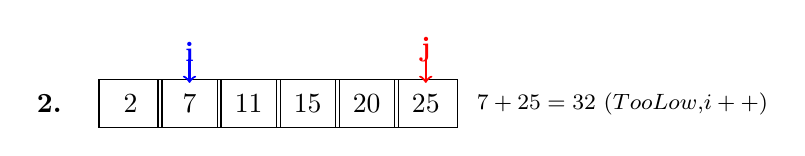
\begin{tikzpicture}[scale=0.75]
        \node[left] at (-0.5,0.35) {\textbf{2.}};
        \foreach \x/\val in {0/2,1/7,2/11,3/15,4/20,5/25}
            \node[draw, minimum width=0.8cm, minimum height=0.6cm] at (\x+0.5,0.35) {\val};
        \draw[->, blue, thick] (1.5,1.1) -- (1.5,0.7) node[above=4pt] {\bf i};
        \draw[->, red, thick] (5.5,1.1) -- (5.5,0.7) node[above=4pt] {\bf j};
        \node[right] at (6.2, 0.35) {\footnotesize $7+25=32 \ (\text{Too Low, } i++)$};
    \end{tikzpicture}

    \pause
    \vspace{0.2cm}
    % Iteration 3
    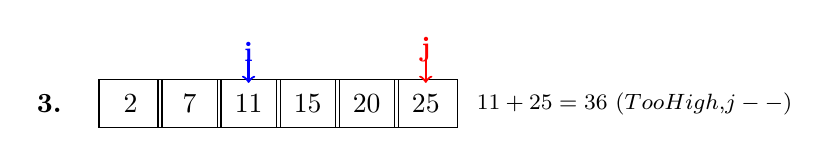
\begin{tikzpicture}[scale=0.75]
        \node[left] at (-0.5,0.35) {\textbf{3.}};
        \foreach \x/\val in {0/2,1/7,2/11,3/15,4/20,5/25}
            \node[draw, minimum width=0.8cm, minimum height=0.6cm] at (\x+0.5,0.35) {\val};
        \draw[->, blue, thick] (2.5,1.1) -- (2.5,0.7) node[above=4pt] {\bf i};
        \draw[->, red, thick] (5.5,1.1) -- (5.5,0.7) node[above=4pt] {\bf j};
        \node[right] at (6.2, 0.35) {\footnotesize $11+25=36 \ (\text{Too High, } j--)$};
    \end{tikzpicture}

    \pause
    \vspace{0.2cm}
    % Iteration 4
    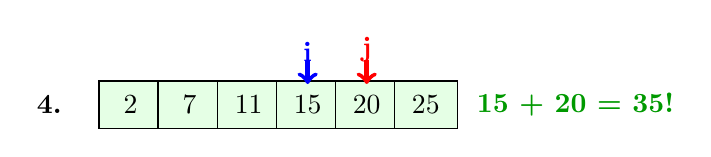
\begin{tikzpicture}[scale=0.75]
        \node[left] at (-0.5,0.35) {\textbf{4.}};
        \foreach \x/\val in {0/2,1/7,2/11,3/15,4/20,5/25}
            \node[draw, minimum width=0.8cm, minimum height=0.6cm, fill=green!10] at (\x+0.5,0.35) {\val};
        \draw[->, blue, ultra thick] (3.5,1.1) -- (3.5,0.7) node[above=4pt] {\bf i};
        \draw[->, red, ultra thick] (4.5,1.1) -- (4.5,0.7) node[above=4pt] {\bf j};
        \node[right] at (6.2, 0.35) {\bf \textcolor{green!60!black}{15 + 20 = 35!}};
    \end{tikzpicture}
\end{frame}

\begin{frame}[fragile]{Problem 2: Container With Most Water}
    \textbf{Goal:} Find two lines that together with the x-axis forms a container, such that the container contains the most water.

    \begin{columns}[T]
        \begin{column}{0.45\textwidth}
            \begin{block}{The Algorithm}
            \small
            \begin{enumerate}
                \item $i = 0, j = n-1$.
                \item $Area = \min(h[i], h[j]) \times (j - i)$.
                \item Update $maxArea$ if current is larger.
                \item \textbf{Crucial:} Move the pointer pointing to the \textbf{shorter} line.
            \end{enumerate}
            \end{block}
            
            \begin{block}{Complexity}
            \small
            \begin{itemize}
                \item \textbf{Time:} $O(N)$
                \item \textbf{Space:} $O(1)$
            \end{itemize}
            \end{block}
        \end{column}

        \begin{column}{0.52\textwidth}
            \begin{exampleblock}{Kotlin Implementation}
\begin{lstlisting}[language=Kotlin, basicstyle=\tiny\ttfamily, keywordstyle=\color{blue}]
fun maxArea(height: IntArray): Int {
    var max = 0
    var i = 0
    var j = height.size - 1
    
    while (i < j) {
        val h = minOf(height[i], height[j])
        val w = j - i
        max = maxOf(max, h * w)
        
        if (height[i] < height[j]) i++
        else j--
    }
    return max
}
\end{lstlisting}
            \end{exampleblock}
        \end{column}
    \end{columns}
\end{frame}

\begin{frame}{Container With Most Water: Trace}
    \centering
    \textbf{Heights: [1, 8, 6, 2, 5, 4, 8]} \quad \textbf{Max Area: \textcolor{green!60!black}{40}}
    \vspace{0.2cm}

    \begin{columns}[T]
        \begin{column}{0.5\textwidth}
            \centering
            % Iteration 1
            \textbf{Step 1: Initial State} \\
            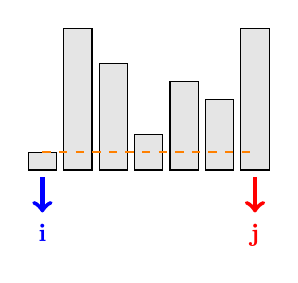
\begin{tikzpicture}[scale=0.45]
                \foreach \x/\h in {0/1, 1/8, 2/6, 3/2, 4/5, 5/4, 6/8}
                    \draw[fill=gray!20] (\x,0) rectangle (\x+0.8, \h/2);
                \draw[blue, ultra thick, ->] (0.4, -0.2) -- (0.4, -1.2) node[below] {\small \bf i};
                \draw[red, ultra thick, ->] (6.4, -0.2) -- (6.4, -1.2) node[below] {\small \bf j};
                \draw[dashed, orange, thick] (0.4, 0.5) -- (6.4, 0.5);
            \end{tikzpicture} \\
            \footnotesize $W=6, H=1 \rightarrow \mathbf{Area=6}$ \\
            \tiny \textcolor{blue}{$h[i] < h[j] \implies i++$}
            
            \pause
            \vspace{0.4cm}
            
            % Iteration 2
            \textbf{Step 2: Found Max} \\
            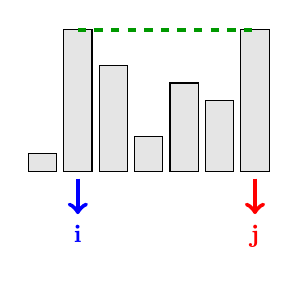
\begin{tikzpicture}[scale=0.45]
                \foreach \x/\h in {0/1, 1/8, 2/6, 3/2, 4/5, 5/4, 6/8}
                    \draw[fill=gray!20] (\x,0) rectangle (\x+0.8, \h/2);
                \draw[blue, ultra thick, ->] (1.4, -0.2) -- (1.4, -1.2) node[below] {\small \bf i};
                \draw[red, ultra thick, ->] (6.4, -0.2) -- (6.4, -1.2) node[below] {\small \bf j};
                \draw[dashed, green!60!black, ultra thick] (1.4, 4) -- (6.4, 4);
            \end{tikzpicture} \\
            \footnotesize $W=5, H=8 \rightarrow \mathbf{Area=40}$ \\
            \tiny \textcolor{red}{$h[j] \le h[i] \implies j--$}
        \end{column}

        \pause
        \begin{column}{0.5\textwidth}
            \centering
            % Iteration 3
            \textbf{Step 3: Trying for more...} \\
            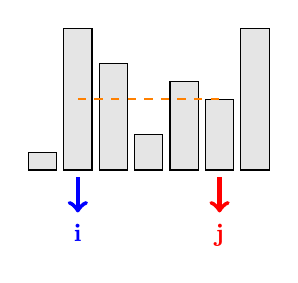
\begin{tikzpicture}[scale=0.45]
                \foreach \x/\h in {0/1, 1/8, 2/6, 3/2, 4/5, 5/4, 6/8}
                    \draw[fill=gray!20] (\x,0) rectangle (\x+0.8, \h/2);
                \draw[blue, ultra thick, ->] (1.4, -0.2) -- (1.4, -1.2) node[below] {\small \bf i};
                \draw[red, ultra thick, ->] (5.4, -0.2) -- (5.4, -1.2) node[below] {\small \bf j};
                \draw[dashed, orange, thick] (1.4, 2) -- (5.4, 2);
            \end{tikzpicture} \\
            \footnotesize $W=4, H=4 \rightarrow \mathbf{Area=16}$ \\
            \tiny \textcolor{green!60!black}{Max remains 40}

            \pause
            \vspace{0.8cm}
            \begin{block}{Intuition}
                \scriptsize
                Moving the taller pointer can only decrease area (width shrinks and height is capped by the shorter side). We \textbf{must} move the shorter pointer to find a taller container.
            \end{block}
        \end{column}
    \end{columns}
\end{frame}

\begin{frame}{Container With Most Water: Iteration 1}
    \centering
    \textbf{Heights: [1, 8, 6, 2, 5, 4, 8]}
    \vspace{0.8cm}

    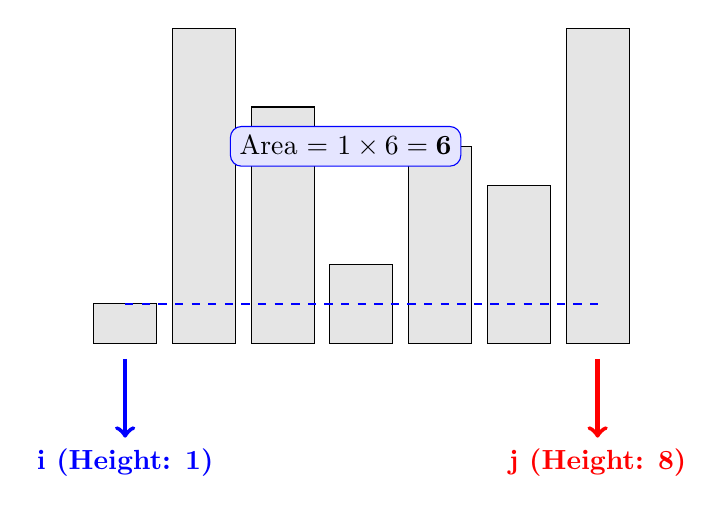
\begin{tikzpicture}[scale=1.0]
        \foreach \x/\h in {0/1, 1/8, 2/6, 3/2, 4/5, 5/4, 6/8}
            \draw[fill=gray!20] (\x,0) rectangle (\x+0.8, \h/2);
            
        \draw[blue, ultra thick, ->] (0.4, -0.2) -- (0.4, -1.2) node[below] {\bf i (Height: 1)};
        \draw[red, ultra thick, ->] (6.4, -0.2) -- (6.4, -1.2) node[below] {\bf j (Height: 8)};
        
        \draw[dashed, blue, thick] (0.4, 0.5) -- (6.4, 0.5);
        \node[fill=blue!10, draw=blue, rounded corners] at (3.2, 2.5) {Area = $1 \times 6 = \mathbf{6}$};
    \end{tikzpicture}

    \begin{block}{Logic}
        $h[i] < h[j]$ (1 < 8). To find a larger area, we move the \textbf{shorter} pointer. \\
        Action: \textbf{Increment $i$}
    \end{block}
\end{frame}